\section{Experimental evidence and its limits}\label{sec:experiments}

The experiments test equivalence of bounded searches, independent replay,
the default localization radius, and the cost of repeated overlap. They
do not measure a complete knot-recognition pipeline. All raw data, source
digests, generated fixtures, and replay commands are retained.

\subsection{Genuine upward-required solid-torus fixtures}

Start with a one-tetrahedron layered solid torus and attach a chain of $g$
copies of the six-tetrahedron ball along boundary triangles. Attaching a
ball along a boundary disc preserves the solid torus. The resulting source
has $t=6g+1$ tetrahedra. Its cocycle is computed and validated using the
maintained exact native routines. Independent Regina checks confirm validity,
orientability, and the solid-torus type for the controlled small instances
\cite{regina}.

These sources have no initial downward move; the native move inventory has
$8g$ upward choices. A local first descent requires one upward and two
downward moves and consumes six original gadget cells. For the one-gadget
source the complete $U=0$ test fails to descend, and the complete
$U=1,r=5$ covered search also fails. With $U=1,r=6$, the native search
returns an independently accepted descent. This distinguishes a genuinely
upward-required test from an example solved by an initial greedy collapse.
The separate ball proof and Regina inventory establish the sharper
radius statement of \cref{prop:sharp}.

\subsection{Matched timing protocol}

The retained measurements use Python 3.12.14 on
\code{Linux-6.18.44-x86_64-with-glibc2.39}. Every source is constructed once.
The independent controls use Regina engine 7.4 (Python package 7.4.1).
Both routes use the same $U=1,r=6$, cochain, native move and transport
routines, and relevant resource limits. Disc queries are disabled.
Each reported time is the median of three retained samples; the run order
alternates between restarted and shared search. The speed ratio is the
ratio of those two medians, not the median of per-pair ratios.

For complete-family timings, endpoint collection is disabled in both
routes. Endpoint equality is checked separately. For first-descent timings,
both routes include the same independent positive verifier. Source fixture
construction is outside the timed calls, while region enumeration and
index construction are inside. Timing uses a shared execution environment,
without dedicated CPU isolation. Three samples document a reproducible
finite comparison but do not support a population confidence interval or
an extrapolated running-time law.

\begin{table}[ht]
\centering\small
\begin{tabular}{@{}rrrrrrrr@{}}
\toprule
$t$ & Covers & \multicolumn{2}{c}{Visited frames} &
\multicolumn{2}{c}{Median seconds} & Ratio & Endpoints\\
\cmidrule(lr){3-4}\cmidrule(lr){5-6}
& & Restart & Shared & Restart & Shared & & \\
\midrule
7  & 66  & 495  & 28 & 1.15956  & 0.09137 & $12.69\times$ & 14\\
13 & 334 & 3152 & 55 & 13.39354 & 0.22377 & $59.85\times$ & 27\\
\bottomrule
\end{tabular}
\caption{Complete covered-family exhaustion. ``Endpoints'' counts exact
signed-cochain geometric isomorphism classes, checked outside the timed
runs. The shared search retains more marked representatives.}
\label{tab:exhaustion}
\end{table}

\begin{table}[ht]
\centering\small
\begin{tabular}{@{}rrrrrrr@{}}
\toprule
$t$ & Covers & \multicolumn{2}{c}{Visited frames} &
\multicolumn{2}{c}{Median seconds} & Ratio\\
\cmidrule(lr){3-4}\cmidrule(lr){5-6}
& & Restart & Shared & Restart & Shared & \\
\midrule
7  & 66   & 273 & 6 & 0.71148  & 0.01801 & $39.50\times$\\
13 & 334  & 630 & 6 & 2.75100  & 0.03303 & $83.29\times$\\
25 & 934  & 641 & 6 & 6.03841  & 0.10123 & $59.65\times$\\
49 & 2134 & 641 & 6 & 10.68172 & 0.14371 & $74.33\times$\\
\bottomrule
\end{tabular}
\caption{First independently verified strict descent on the controlled
solid-torus family. Every selected witness uses one upward and two downward
moves. These are simplifier measurements, not end-to-end unknot timings.}
\label{tab:descent}
\end{table}

\begin{figure}[ht]
\centering
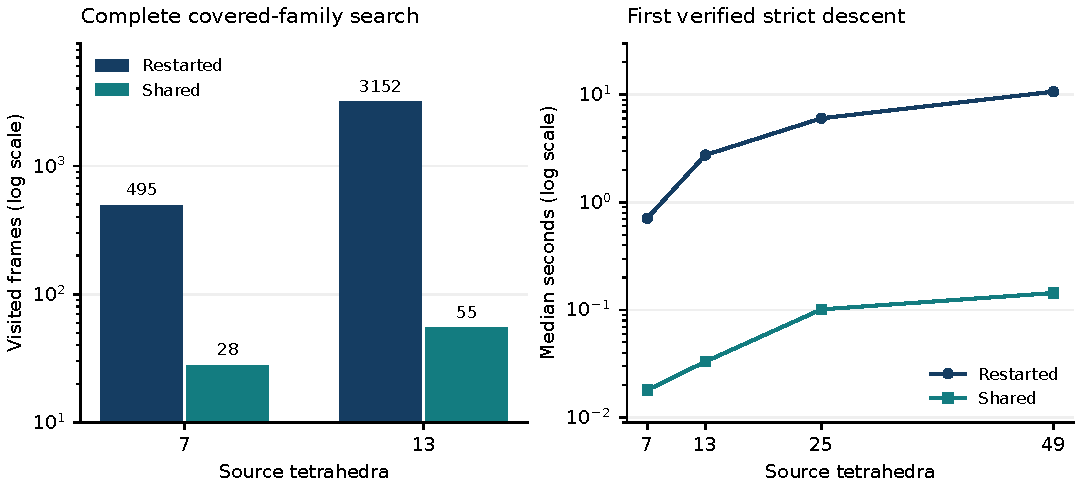
\includegraphics[width=\textwidth]{figures/benchmarks.pdf}
\caption{Two views of the same retained data. Logarithmic vertical axes
make the smaller shared-search counts and times legible. Lines connect
the four measured first-descent cases and do not represent a fitted
asymptotic model.}
\label{fig:benchmark}
\end{figure}

In the complete runs, cooperative work checkpoints fall from $367{,}010$
to $23{,}374$ at $t=7$, and from $4{,}136{,}232$ to $84{,}460$ at $t=13$.
The changes are consistent with removing repeated common prefixes across
overlapping covers. In the first-descent runs the shared method visits
six frames and materializes five transitions; its selected proof has
three events, so two materialized transitions belong to unsuccessful
visited alternatives. Lazy materialization avoids paying for the unvisited
siblings. Constant visited-frame counts do not imply constant runtime:
the cover index and global geometry still grow with the source.

\subsection{Exact endpoint equality and standalone replay}

For $t=7$ and $t=13$, complete restarted and shared enumeration produce
identical sets of full exact signed-cochain isomorphism tuples: respectively
$14$ and $27$ classes. This comparison forgets source incarnation names
but retains the geometric face-pairing structure and integral marking.
The shared search retains $28$ and $55$ marked endpoints. Thus the audit
does not claim that the two implementations visit identical histories or
have a pointwise bijection between their internal frames.

Independent source-bound replay separately authenticates reachability and
scope. The complete-family artifact's standalone replay accepts $124$
retained covered endpoint certificates and six strict-descent certificates.
The first-descent artifact's replay accepts another twelve strict descents.
These counts include retained representatives and repeated timing witnesses
according to the artifact schema; they are not numbers of distinct knot
types or geometric states.

\subsection{Adversarial and combinatorial audits}

The targeted cover tests compare inverted-index intersections with literal
subset containment, compare complete endpoint families against both older
restarted and naive routes, and exercise independent replay with producers
disabled. They distinguish actual support from a supplied connected cover,
including a disconnected consumed subset. They test incomplete indexing,
exact work boundaries, a one-node cap before transport, callback mutation
isolation, and propagation of exceptions raised while converting a callback
result to a truth value.

The causal tests cover independent event components, positive projection,
the late-merger case that requires repeated projection and truncation,
invalid or non-descending inputs, and declared noncanonical downward
frames. The portable frame audit constructs $144$ formal variants on two
dependent downward steps from fixed verified data and explicit cell/vertex
renamings. Every input and extracted output passes independent replay;
the exact final triangulation, normalized marking, and coherent coordinates
agree in every case. In $48$ variants the final seed is a child of the
preceding downward move, directly exercising the frame-sensitive dependency.
No search or Pachner producer constructs those input variants.

The colorful-packing tests compare every subset of $96$ deterministic
random item families under four budget/goal choices. They also test zero-cost
items, empty inputs, invalid or repeated footprints, color-label compaction,
discarded-item index preservation, and exact witness reconstruction after
profit capping. On the genuine two-gadget source, all $55$ retained endpoints
are independently replayed and yield six positive candidates: three on
each of the disjoint six-cell supports. One supplied coloring permits
packing two items with total upward cost two and loss two. An exhaustive
check of all $64$ subsets finds nine optimal pairs and agrees with the DP.

The composition audit then replays a selected pair and produces a single
certificate for $13\to11$ tetrahedra with $u=2,d=4$. Independent replay
accepts both source proofs and the composed proof. Tests also reverse the
order, allow overlapping declared covers with disjoint actual supports,
reject overlapping actual supports and forged evidence, preserve
noncanonical frames, and exercise empty composition and exact work limits.
A further portable audit constructs twelve paired belt/apex frame variants
of the second nonempty input trace and composes them after the first trace
has changed row positions. Every composed endpoint verifies with the
correct private birth namespaces and additive counts. These twelve focused
composition cases are distinct from the exhaustive $144$-frame extraction
audit.

Three implementation issues found during development are retained as regression
targets. An eager branch producer did unnecessary sibling transport before
the next node-limit check; deferred materialization fixes this. A causal
replay initially assumed the native producer's downward frame was the only
verified frame; preserving the certificate's declared frame fixes the
dependent-step failure. The cover search also now shields the truth-value
conversion of an endpoint callback result, so a callback exception cannot
be mistaken for an internal work-limit signal. These corrections improve the trust boundary as
well as measured performance.

\subsection{Complete regression and reproducibility}

The complete current inventory contains $1483$ tests in $187$ modules; all
pass with zero failures, errors, or skips. Verification uses six fresh
interpreter batches. After adapting one incoming test to the newer native
unit-ray optimization, the affected fifth batch ($315$ tests) was rerun
successfully. Source hashes confirm that the other tested modules and every
production module were unchanged.

The initial runner required an explicit import path for inherited test
helpers. Its failed setup record, the corrected run, the compatibility
patch, and the successful affected-batch rerun are retained. The adapted
test separately checks the native zero-orbit optimization and forces the
documented fallback schedule to preserve the original exact-budget and
under-budget assertions. No native production file was replaced or altered.
The final machine-readable aggregate lists every test ID, its batch evidence,
and current source hashes; it does not erase the earlier diagnostic runs.


Run the principal checks from the delivered \code{repro/fast} directory:
\begin{lstlisting}[language=bash]
python -m unittest tests.test_pachner_cover_search \
  tests.test_pachner_causality tests.test_pachner_composition \
  tests.test_colorful_packing -v
python -m shared_cover_research.benchmark \
  --replay shared_cover_research/results/exhaustion.json
python -m shared_cover_research.benchmark \
  --replay shared_cover_research/results/descent.json
python -m causal_research.composition_audit \
  --replay causal_research/results/disjoint_composition.json \
  --output reproduced/composition_replay.json
\end{lstlisting}
The package-level regression runner discovers the complete delivered test
inventory, records hashes and test IDs, and runs six fresh interpreters.
Fresh output directories keep reproduction results separate from recorded
evidence. The frame and ball audit drivers, paired benchmark generator,
figure generator, and checksum verifier have their own documented commands.

\subsection{What the evidence establishes}

\begin{table}[ht]
\centering\small
\begin{tabularx}{\textwidth}{@{}p{0.36\textwidth}X@{}}
\toprule
Claim & Basis and present scope\\
\midrule
Connected footprint $\le3U+3$ & General proof in the stated move category;
sharp at $U=1$ by a separate proof and finite inventory.\\
$2^{O(U)}\poly(t+B)$ descent & Complete deterministic algorithm with explicit
region and trace counting; implemented via shared sleep search.\\
$2^{O(U+k)}\poly(t+B)$ multiunit descent & General proof using a cited perfect
hash family; supplied-coloring DP and positive composition implemented.\\
Faster covered search & Exact endpoint agreement and paired finite timings
on constructed valid solid tori.\\
General quasi-polynomial ProveIt recognition & Conditional on the additional
structural and terminal hypotheses in \cref{thm:conditional}.\\
\bottomrule
\end{tabularx}
\caption{Proof, implementation, and empirical claims are stated separately.}
\end{table}

The benchmark family was designed to isolate repeated cover work. It does
not sample arbitrary knot exteriors, establish favorable average behavior,
or show that the worst-case exponential constants are small. The explicit
index can be a poor practical choice when few covers are useful or memory
is scarce. These limitations motivate the broader census and index work in
\cref{sec:questions}; they do not weaken the complete bounded decision
theorems, whose correctness and asymptotic scope come from the proofs.
